\documentclass[main.tex,fontsize=8pt,paper=a4,paper=portrait,DIV=calc,]{scrartcl}
% Document
\usepackage[T1]{fontenc}
\usepackage[utf8]{inputenc}
\usepackage[dvipsnames]{xcolor}
\usepackage[nswissgerman,english]{babel} 
\usepackage{hyperref}
\renewcommand{\familydefault}{\sfdefault}

% Format
\usepackage[top=5mm,bottom=1mm,left=5mm,right=5mm]{geometry}
%\setlength{\headheight}{\baselineskip}
%\setlength{\headsep}{0mm}

%\usepackage{scrlayer-scrpage}
%\clearpairofpagestyles
%\chead{{\bfseries\TITLE, \AUTHOR, \pagename~\thepage}}

%\addtokomafont{pagehead}{\upshape}

\usepackage{multicol}
\setlength{\columnsep}{2mm}
\setlength{\columnseprule}{0.1pt}

% Math
\usepackage{amsmath}
\usepackage{amssymb}
\usepackage{amsfonts}

% Code
\usepackage{fancyvrb, etoolbox, listings, xcolor}
%\usemintedstyle{bw}

%\newminted[shell]{bash}{
%fontsize=\footnotesize,
%fontfamily=tt,
%breaklines=true,
%frame=single,
%framerule=0.1pt,
%framesep=2mm,
%tabsize=2
%}
%\newminted{css}{
%breaklines=true,
%tabsize=4,
%autogobble=true,
%escapeinside=||,
%stripall=true,
%stripnl=true,
%}

    \definecolor{lightgray}{rgb}{0.95, 0.95, 0.95}
    \definecolor{darkgray}{rgb}{0.4, 0.4, 0.4}
    \definecolor{purple}{rgb}{0.65, 0.12, 0.82}
    \definecolor{ocherCode}{rgb}{1, 0.5, 0} % #FF7F00 -> rgb(239, 169, 0)
    \definecolor{blueCode}{rgb}{0, 0, 0.93} % #0000EE -> rgb(0, 0, 238)
    \definecolor{greenCode}{rgb}{0, 0.6, 0} % #009900 -> rgb(0, 153, 0)
    \definecolor{teal}{rgb}{0.0, 0.5, 0.5}

\lstdefinestyle{code}{
    identifierstyle=\color{black},
    keywordstyle=\color{blue}\bfseries\small,
    ndkeywordstyle=\color{greenCode}\bfseries\small,
    stringstyle=\color{ocherCode}\ttfamily\small,
    commentstyle=\color{teal}\ttfamily\textit\small,
    basicstyle=\ttfamily\small,
    breakatwhitespace=false,         
    breaklines=true,                 
    captionpos=b,                    
    keepspaces=true,                 
    showspaces=false,                
    showstringspaces=false,
    showtabs=false,                  
    tabsize=2,
    belowskip=-5pt
}



% Images
\usepackage{graphicx}
\newcommand{\pic}{\includegraphics[scale=0.3]}
\graphicspath{{Screenshots/}{../Screenshots}}
\makeatletter
\def\pictext#1#2{%
    \@ifnextchar[{%
    \pictext@iiiii{#1}{#2}%
    }{%
      \pictext@iiiii{#1}{#2}[0.5,0.4,0.3]% Default is 5
    }%
}
\def\pictext@iiiii#1#2[#3,#4,#5]{\begin{minipage}{#3\textwidth}\includegraphics[scale=#4]{#1}\end{minipage}\begin{minipage}{#5\textwidth}#2\end{minipage}}
\def\minipg#1#2{%
    \@ifnextchar[{%
    \minipg@iiii{#1}{#2}%
    }{%
      \minipg@iiii{#1}{#2}[0.3,0.6]% Default is 5
    }%
}
\def\minipg@iiii#1#2[#3,#4]{\vspace{0.8mm}\begin{minipage}{#3\textwidth}#1\end{minipage}\begin{minipage}{#4\textwidth}#2\end{minipage}{\vspace{0.8mm}}}
\makeatother

%\newenvironment{minty}[2]% environment name
%{% begin code
%  \begin{minipage}{#1}
%  \begin{minted}{#2}
%}%
%{% end code
%  \end{minted}
%  \end{minipage}
%  \end{minty}\ignorespacesafterend
%} 

% Smaller Lists
\usepackage{enumitem}
\setlist[itemize,enumerate]{leftmargin=3mm, labelindent=0mm, labelwidth=1mm, labelsep=1mm, nosep}
\setlist[description]{leftmargin=0mm, nosep}
\setlength{\parindent}{0cm}

% Smaller Titles
\usepackage[explicit]{titlesec}

%% Color Boxes
\newcommand{\sectioncolor}[1]{\colorbox{black!60}{\parbox{0.989\linewidth}{\color{white}#1}}}
\newcommand{\subsectioncolor}[1]{\colorbox{black!50}{\parbox{0.989\linewidth}{\color{white}#1}}}
\newcommand{\subsubsectioncolor}[1]{\colorbox{black!40}{\parbox{0.989\linewidth}{\color{white}#1}}}
\newcommand{\paragraphcolor}[1]{\colorbox{black!30}{\parbox{0.989\linewidth}{\color{white}#1}}}
\newcommand{\subparagraphcolor}[1]{\colorbox{black!20}{\parbox{0.989\linewidth}{\color{white}#1}}}

%% Title Format
\titleformat{\section}{\vspace{0.5mm}\bfseries}{}{0mm}{\sectioncolor{\thesection~#1}}[{\vspace{0.5mm}}]
\titleformat{\subsection}{\vspace{0.5mm}\bfseries}{}{0mm}{\subsectioncolor{\thesubsection~#1}}[{\vspace{0.5mm}}]
\titleformat{\subsubsection}{\vspace{0.5mm}\bfseries}{}{0mm}{\subsubsectioncolor{\thesubsubsection~#1}}[{\vspace{0.5mm}}]
\titleformat{\paragraph}{\vspace{0.5mm}\bfseries}{}{0mm}{\paragraphcolor{\theparagraph~#1}}[{\vspace{0.5mm}}]
\titleformat{\subparagraph}{\vspace{0.5mm}\bfseries}{}{0mm}{\subparagraphcolor{\thesubparagraph~#1}}[{\vspace{0.5mm}}]

%% Title Spacing
\titlespacing{\section}{0mm}{0mm}{0mm}
\titlespacing{\subsection}{0mm}{0mm}{0mm}
\titlespacing{\subsubsection}{0mm}{0mm}{0mm}
\titlespacing{\paragraph}{0mm}{0mm}{0mm}
\titlespacing{\subparagraph}{0mm}{0mm}{0mm}

%% format cells
\usepackage[document]{ragged2e}
\usepackage{array, makecell}
\renewcommand{\arraystretch}{2}
\newcommand{\mc}{\makecell[{{m{1\linewidth}}}]}



\lstset{
    language={[x86masm]Assembler},
    style=code,
}

\begin{document}
\tableofcontents

\newcommand{\TITLE}{Secure Software}
\newcommand{\AUTHOR}{Fabio Lenherr}
\setcounter{tocdepth}{1}

\section{Secure Software Principles}
\textcolor{Cyan}{Rather than trying to solve objectives in cyber security, you should have expectations of your software in terms of security.}

\subsection{CVSS Common Vulnerability Scoring System}
\begin{itemize}
  \item \textcolor{red}{High}\newline
    Heartbleed, log4j etc\newline
    often not noticeable, concealed
  \item \textcolor{blue}{Medium}\newline
    unclear if it can be exploited
  \item \textcolor{green}{Low}\newline
    typical problems like outdated tls certificate
\end{itemize}

\subsection{Low-hanging fruits first}
\textcolor{teal}{Before we go ahead and tackle the biggest issues, we can solve a lot of problems by making sure that we do not fail at the basics.}\newline
In other words, first try to solve the easy things.

\subsection{80\%/20\% Problem}
\begin{itemize}
\item \textcolor{purple}{Secure the weakest link}\newline
  A boomer might not know about phishing attacks, protect said user against doing something dumb!
\item \textcolor{purple}{Practice defense in depth}\newline
  Use multiple security layers, often 1 is not enough
\item \textcolor{purple}{Fail secure}\newline
  In terms of an error, don't just dump all information to some random person, eg. don't leak credit card information if the information is not 100\% correct.
\item \textcolor{purple}{Follow the principle of least privilege}\newline
  Don't give random people access to things they don't need
\item \textcolor{purple}{To Compartmentalize}\newline
  Try to categorize tasks, this makes it easier for people to get access to something.
\item \textcolor{purple}{Keep it simple}\newline
  Try to keep it as simple as possible
\item \textcolor{purple}{Promote privacy}\newline
  Handle privacy of users appropriately
\item \textcolor{purple}{Remember that hiding secrets is hard}
  In other words, security by obscurity is a novel practice and doesn't really work
\item \textcolor{purple}{Be reluctant to trust}
\item \textcolor{purple}{Use your community resources}
\end{itemize}

\section{Threat Models \& Mitigations}
\subsection{The 4 Questions}
\begin{enumerate}
\item \textcolor{purple}{What are we working on?}\newline
  \begin{itemize}
  \item \textcolor{black}{Define scope and context}
  \item \textcolor{black}{Description of requirements and design}
  \end{itemize} 
\item \textcolor{purple}{What can go wrong?}\newline
  Anciticapte potential issues (think like the attacker)
\item \textcolor{purple}{What are we going to do about it?}\newline
  Define mitigations
\item \textcolor{purple}{Did we do a good job?}\newline
  Reflection and confirmation
\end{enumerate} 

\subsection{Methodology for Threat Risk Modeling}
\begin{enumerate}
\item \textcolor{purple}{Identify security objectives with a focus on:}\newline
 \begin{itemize}
 \item \textcolor{black}{sensitive information stored on device}
 \item \textcolor{black}{third party libraries used}
 \item \textcolor{black}{loss of repudation derived from misuse of the application}
 \end{itemize} 
\item \textcolor{purple}{Break down the application features, i.e. decomposition of the application into small feature sets with the goal to identify security impact}
\item \textcolor{purple}{Identification of related threats and vulnerabilities in implementation}
\end{enumerate} 

\subsection{Process Steps}
\begin{enumerate}
\item \textcolor{purple}{Identity Assets}\newline
What do we own and what do we want to protect? Not everything is worth protecting!
\item \textcolor{purple}{Create an architecture overview}\newline
  Simple diagrams which include application, subsystems, trust boundaries and data flow
\item \textcolor{purple}{Decompose the application}\newline
  The structure of your application -> network model, API, etc that can lead to potential vulnerabilities
\item \textcolor{purple}{Identify the threats}\newline
  From the attackers perspective, try to find loopholes etc to attack your application and \emph{document them}
\item \textcolor{purple}{Document the threats}\newline
\item \textcolor{purple}{Rate the threats} \newline
  Rate the threats according to \emph{likelihood, impact damage (reputation, cost), damage of migitation (cost, annoyance or work)}
\end{enumerate} 

\subsection{Why?}
The reason we do all this is that the following 3 groups have the these benefits: 
\begin{itemize}
\item \textcolor{purple}{Developers}\newline
  \begin{itemize}
  \item \textcolor{black}{Know potential threats and develop with them in mind}
  \item \textcolor{black}{priorization of threats to proper mitigations can be taken}
  \end{itemize} 
\item \textcolor{purple}{Penetration Testers}\newline
  \begin{itemize}
  \item \textcolor{black}{Makes sure penetration testers don't waste time testing things that don't matter to you}
  \item \textcolor{black}{Have a decent idea where to start}
  \end{itemize} 
\item \textcolor{purple}{Management}\newline
  \begin{itemize}
  \item \textcolor{black}{Know the risks in their language -> cost}
  \item \textcolor{black}{Don't make stupid decisions against developers etc since they don't understand IT}
  \end{itemize} 
\end{itemize} 

\subsection{STRIDE}
\begin{itemize}
\item \textcolor{purple}{Spoofing}\newline
Using a false identity to gain access to a system.\newline
\textcolor{green}{Mitigation: Authentication} Cookies, Signatures, updates TLS
\item \textcolor{purple}{Tampering}\newline
unauthorized changes/manipulation of data\newline
\textcolor{green}{Mitigation: Integrity} ACLs, Digital Signatures
\item \textcolor{purple}{Repudation}\newline
The ability to deny having performed an attack,\newline
\textcolor{green}{Mitigation: Nonrepudation} Secure logging and auditing, Digital Signatures
\item \textcolor{purple}{Impersonation}\newline
unauthorized revelation of classified(PROPRIETARY) private information.\newline
\textcolor{green}{Mitigation: Confidentiality} Encryption, ACLS
\item \textcolor{purple}{Denial of Service}\newline
Prevent or restrict access to a service by flooding it.\newline
\textcolor{green}{Mitigation: Availability} ACLs, Filtering, Quotas
\item \textcolor{purple}{Elevation of Privilege}\newline
Gaining unauthorized privileges on a system. For example: becoming root as regular user\newline
\textcolor{green}{Mitigation: Authorization} ACLs, Group or role membership, privilege ownership, input validation
\end{itemize} 

\subsubsection{Stride and Thread Modeling}
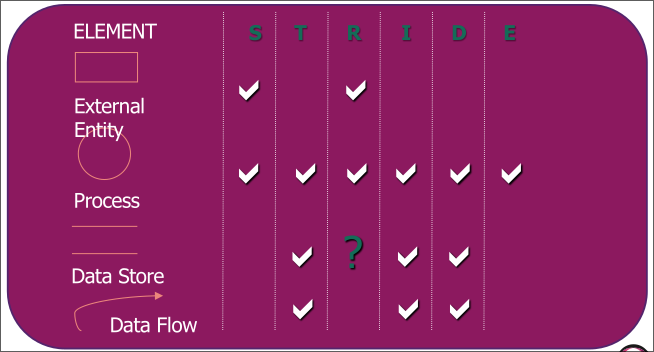
\includegraphics[scale=0.4]{2023_03_02_10_46_31.png}

\subsection{Attack Tree}
This is a list of attacks that can lead to another. This can help with attacks that are \emph{not obvious}.\newline
\textcolor{puple}{Attack trees are complementary to threat modeling}\newline
\textcolor{red}{Here an example of how they work:}\newline
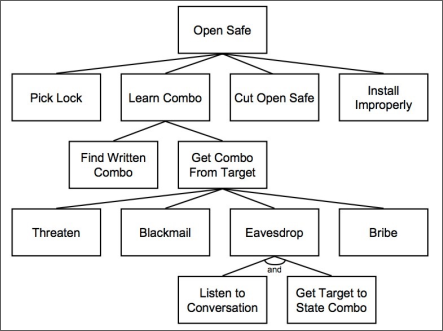
\includegraphics[scale=0.4]{2023_03_02_11_20_47.png}
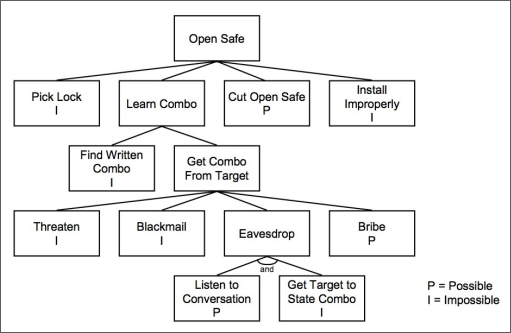
\includegraphics[scale=0.4]{2023_03_02_11_22_00.png}\newline
\textcolor{purple}{Add labels for possible and impossible actions}\newline
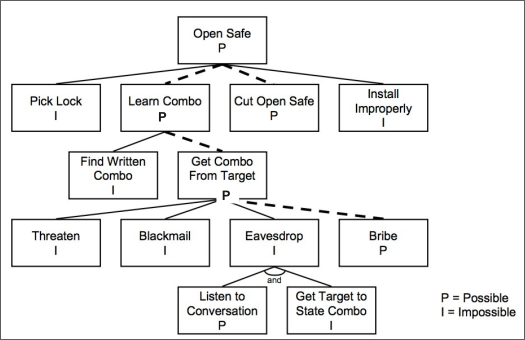
\includegraphics[scale=0.4]{2023_03_02_11_22_15.png}
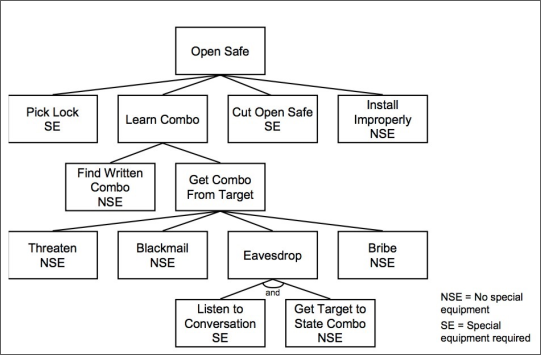
\includegraphics[scale=0.4]{2023_03_02_11_22_25.png}\newline
\textcolor{purple}{Propagate the labels up so possible things are closer, after that \emph{define used tools for the actoins}}\newline
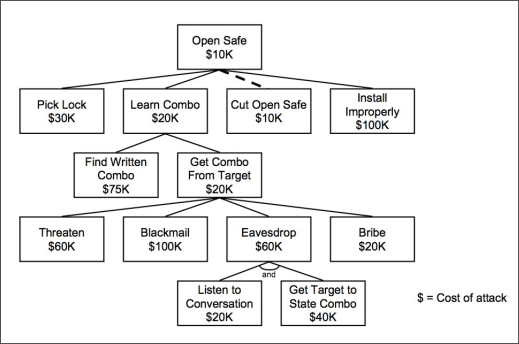
\includegraphics[scale=0.4]{2023_03_02_11_23_15.png}
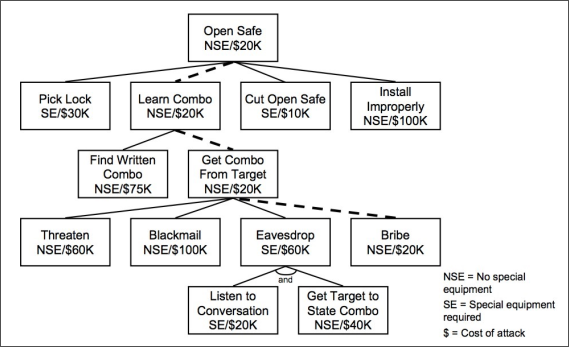
\includegraphics[scale=0.4]{2023_03_02_11_23_34.png}\newline
\textcolor{purple}{Define monetary costs for the attack and \emph{mark the route with least cost and the least tools used}}

\subsection{Risk Management Acitivies}
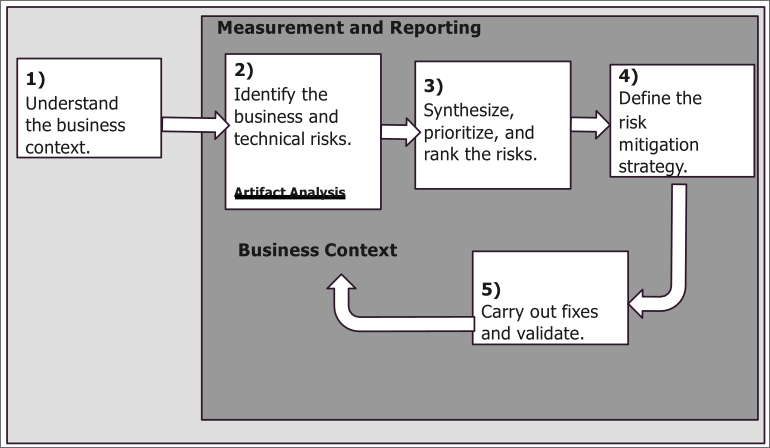
\includegraphics[scale=0.4]{2023_03_02_11_13_47.png}\newline

\section{Software bugs and unexpected behavior}
\subsection{Types of bugs and issues}
\begin{itemize}
\item \textcolor{purple}{security bug}\newline
These are a misimplementation and are easy to discover and remediate using modern code review tools.\newline
Examples include buffer overflows, race conditions and unsafe system calls
\item \textcolor{purple}{security flaw}\newline
This is a design flaw and is hence impossible to detect by automated tools. \newline
This might be bad error handling, type confusion, or just plain wrong usage of something
\item \textcolor{purple}{Decurity defect: security bug + security flaw}
\end{itemize} 

\subsection{Buffer overflow}
\textcolor{purple}{Buffer overflow attacks are common in the C language space. Mostly this is because of use of legacy functions that fail to check for safety.\newline
This can lead to examples where you would like to check a password, however, the attacker provides not just a password, but something longer. When comparing with unsafe code, this could lead to the actual password being overwritten and the attacker therefore gaining access even with a faulty password.}\newline
Here a concrete example for this:
\begin{lstlisting}
#include <stdio.h>
#include <string.h>
void printstr(char *str, int len) {
  for (int i = 0; i < len; i++) {
    printf("%c", str[i]);
  }
  printf("\n");
}

void printstr_unsafe(char *str) {
  int i = 0;
  while (str[i] != '\0') {
    printf("%c", str[i]);
    i++;
  }
  printf("\n");
}

int compstr(char* str1, char* str2, int lower) {
  for(int i = 0; i < lower; i++) {
    // printf("%c", str1[i]);
    // printf("%c", str2[i]);
    if(str1[i] != str2[i]) {
      return 0;
    }
  }
  return 1;
}

int main(int argc, char **argv) {
  int a = 5;
  int b = 7;
  int c = a + b;

  char arr[] = {'g', 'e', 't', 'm', 'e', 'h', 'a', 'c', 'k', 'e', 'd'};
  char arr3[8];
  char arr2[] = "pwsecret";
  
  strcpy(arr3, argv[1]);
  if (compstr(arr2, arr3, 8) == 1) {
    printstr(arr, sizeof(arr));
    return 1;
  }

  printf("you fucked up\n");
  // printstr(arr2, sizeof(arr2));
  // printstr_unsafe(arr2);
  printstr(arr3, sizeof(arr3));   
  printstr(arr2, sizeof(arr2));   

  return 0;
}
\end{lstlisting}
\textcolor{teal}{Note that if the attacker overdoes the length of the malicious string, then the program will read into unallocated memory. This will lead to the OS segfaulting this program.}\newline
\textcolor{red}{Solution: Use modern and secure functions for C/C++ OR use more modern languages such as rust.}

\subsection{Image Visualization of Stack}
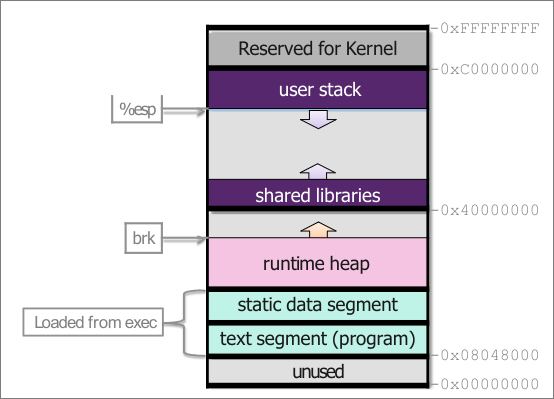
\includegraphics[scale=0.4]{2023_03_16_11_27_16.png}
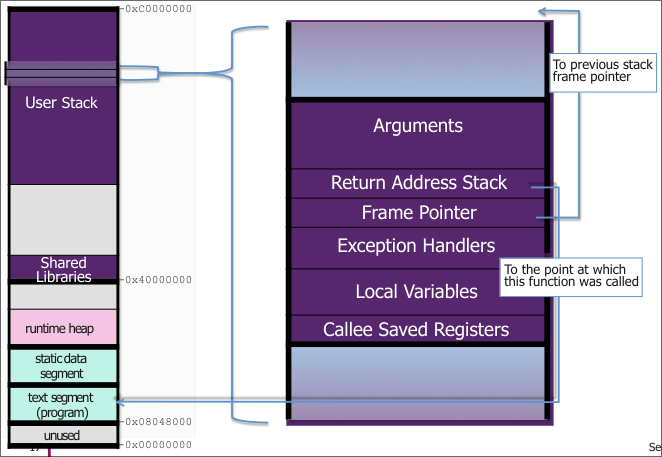
\includegraphics[scale=0.4]{2023_03_16_11_27_42.png}

\subsection{Image Visualization of an attack}
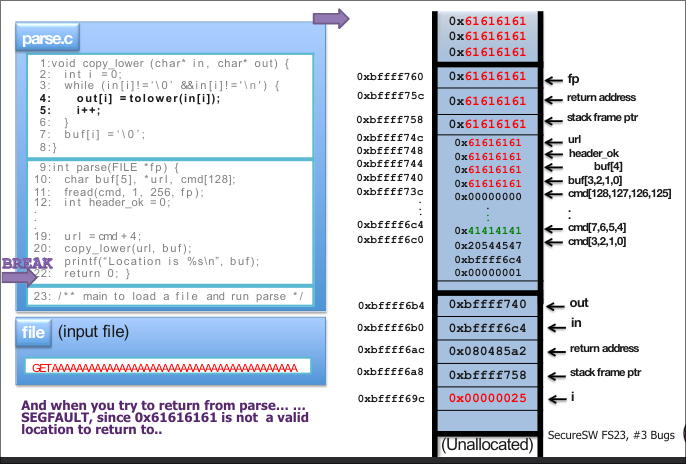
\includegraphics[scale=0.4]{2023_03_16_11_28_24.png}\newline
\textcolor{red}{However, you can just simply create a different return location, since we can override the return address :)}\newline
For this we first have to choose a function to use, let's take execve in order to replace the current program with a shell.\newline
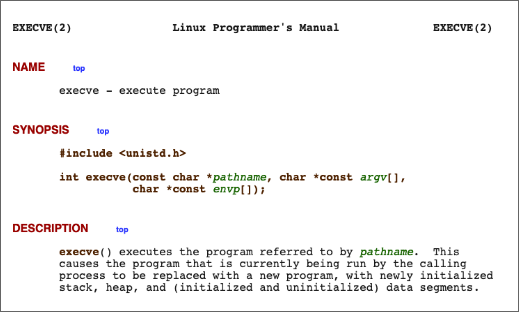
\includegraphics[scale=0.4]{2023_03_16_11_31_03.png}\newline
Then we have to create a main function with a call to execve in order to be able to jump to it.\newline
\textcolor{teal}{Even more important, the function then needs to be disassembled and formatted in order to be used.}\newline
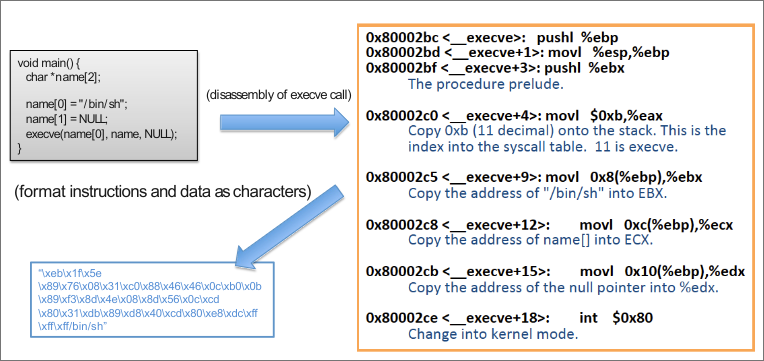
\includegraphics[scale=0.4]{2023_03_16_11_31_59.png}\newline
We can now start to override the return function with this new text.\newline
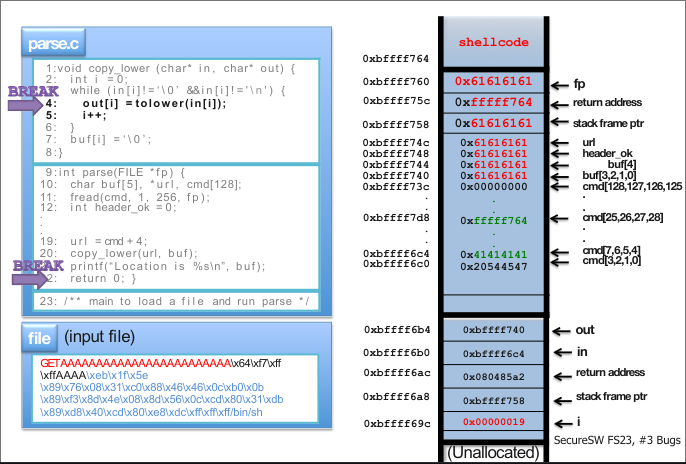
\includegraphics[scale=0.4]{2023_03_16_11_33_05.png}

\subsubsection{NOP}
\textcolor{purple}{The problem we face with return addresses, is that we do not know the exact address that we need to call. This means that we might miss the actual address of our code.\newline
Keep in mind that our address is just offset from the stackpointer. }\newline
\textcolor{teal}{However, there is a solution, we can use NOP instructions as padding around the code. This means that if we jump too high, we will simply run into these NOP statements, which do nothing other than telling the cpu to move to the next statement below.\newline
We can simply repeat this until we are at the evil code.\newline
Should we land below the evil code, then we can use ret statements with an address that is prob above the evil code to run it.}

\section{Concurrency Issues}

\subsection{Race Condition}
This is an access of 2 concurrent processes on a shared state.

\subsection{Critical Section}
This is a part of code, that can lead to race conditions. 

\subsection{ToCToU Time of Check and Time of Use}
For example, before you withdraw money, you need to check if you have enough.\newline
However, in during the time between checking and witdrawing, you have no guarantee that noone else does something with it, without a lock.\newline
This timeframe is the ToCToU.\newline

Example for the issue: \newline
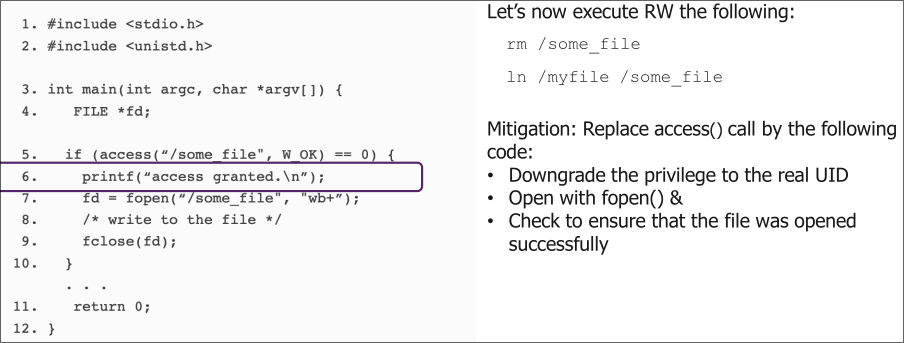
\includegraphics[scale=0.4]{2023_03_23_10_28_49.png}\newline
As you can see, there is a slight timeframe where we can manipulate the file or even link another file so we open another one.\newline
The real userID is the ID of the launching userID -> make sure that no root files can be read.\newline
Another Example:\newline
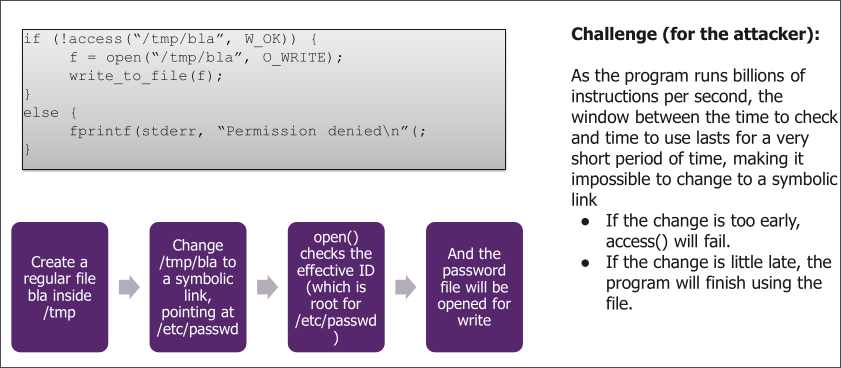
\includegraphics[scale=0.4]{2023_03_23_10_39_39.png}\newline
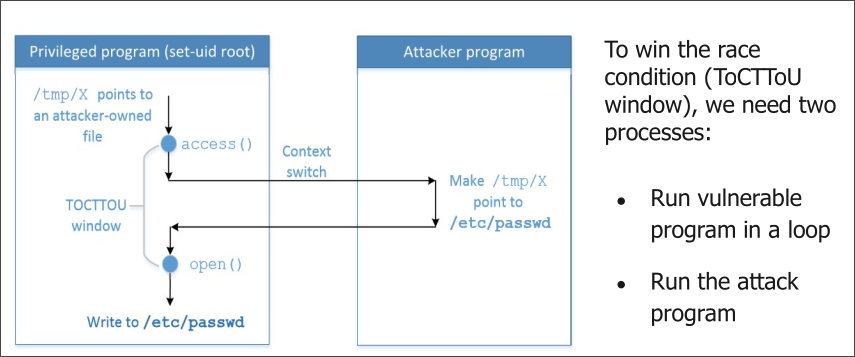
\includegraphics[scale=0.4]{2023_03_23_10_39_50.png}\newline
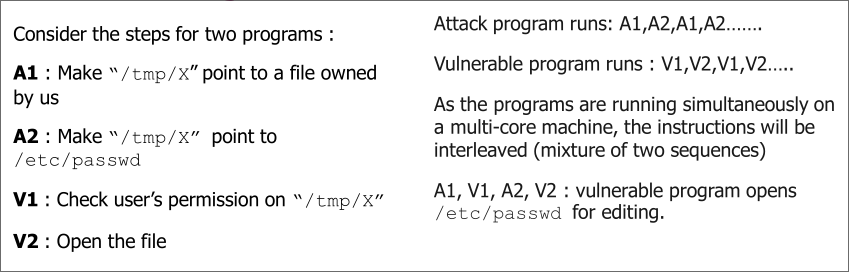
\includegraphics[scale=0.4]{2023_03_23_10_40_02.png}\newline
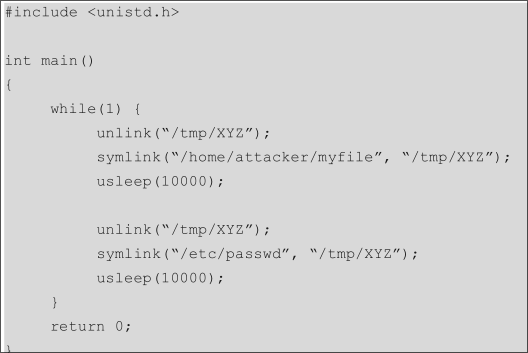
\includegraphics[scale=0.4]{2023_03_23_10_47_01.png}\newline
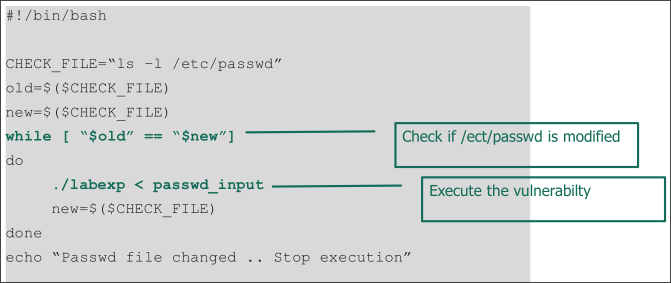
\includegraphics[scale=0.4]{2023_03_23_10_47_12.png}

\subsection{setUID}
This is used for programs that need to run as root, but are launched by the user.\newline
This can be a potential security risk, as can be seen in the subsection above, or in the root shell program in the buffer overflow section!\newline
How to make it work\newline
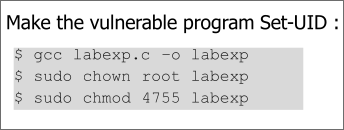
\includegraphics[scale=0.4]{2023_03_23_10_41_37.png}

\subsection{Different Mitigations}
\begin{itemize}
\item \textcolor{purple}{Atomic operations}
\item \textcolor{purple}{Repeating check and use}
\item \textcolor{purple}{Sticky Symlink Protection -> prevent creating symbolic links}
\item \textcolor{purple}{Principles of Least privilege}
\end{itemize} 

\subsection{Atomic Operations}
\begin{lstlisting}
// creates file if not exists
f = open(file, O_CREAT | O_EXCL)
\end{lstlisting}

\subsubsection{Repeating Check ad use}
Here we simply check and open multiple times in order to prevent an attack.\newline
Example, check 2 times, and prevent opening if changed. 

\subsubsection{Sticky Symlink Protection}
\begin{lstlisting}
sudo sysctl -w fs.protected_symlinks=1
\end{lstlisting}
The symlink checks whether or not the user owns either the directory or the symlink.\newline
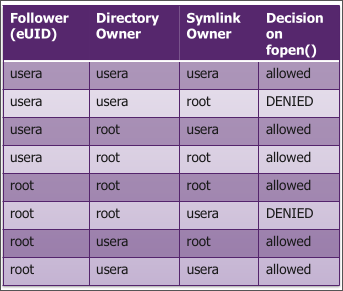
\includegraphics[scale=0.4]{2023_03_23_10_53_20.png}

\subsubsection{Principle of Least Privilege}
The program is using the root UID only, how about we make sure we only use the root UID when we actually need it!\newline
\textcolor{teal}{This can be done with setuid() and seteuid().}
\begin{lstlisting}
uid_t real_uid = getuid(); // get real user id
uid_t eff_uid = getuid(); // get effective user id

seteuid(real_uid); // disable root privilege

f = open("/tmp/XYZ", O_WRITE);
if (f != -1) {
  write_to_file(f);
  } else {
  fprintf(stderr, "Permission denied\n");
}
seteuid(eff_uid); // restore root privilege (if needed)
\end{lstlisting}

\section{Problems with Integers}

\subsection{Integer Promotion}
\begin{lstlisting}
char result,c1,c2,c3;
c1 = 100;
c2 = 90;
c3 = -120;
result = c1 + c2 + c3;
// we would expect a char overflow, however instead they are promoted to integers, as these can store these values.
// at the end we have a char again, as the result is small enough for a char.
// would the endresult be too big, then we would have an overflow!!
\end{lstlisting}

\subsection{Implicit Conversions}
\textcolor{purple}{Unsigned implicit conversion}\newline
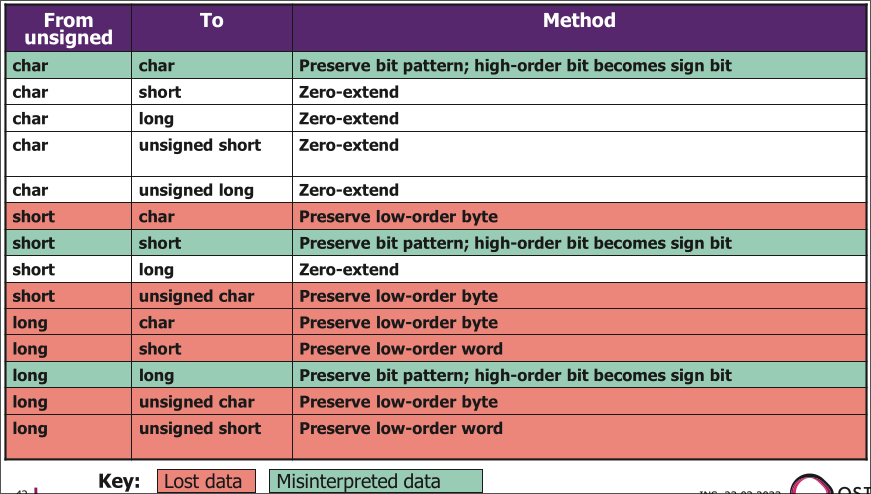
\includegraphics[scale=0.4]{2023_03_23_11_17_02.png}\newline
\textcolor{purple}{Signed implicit conversion}\newline
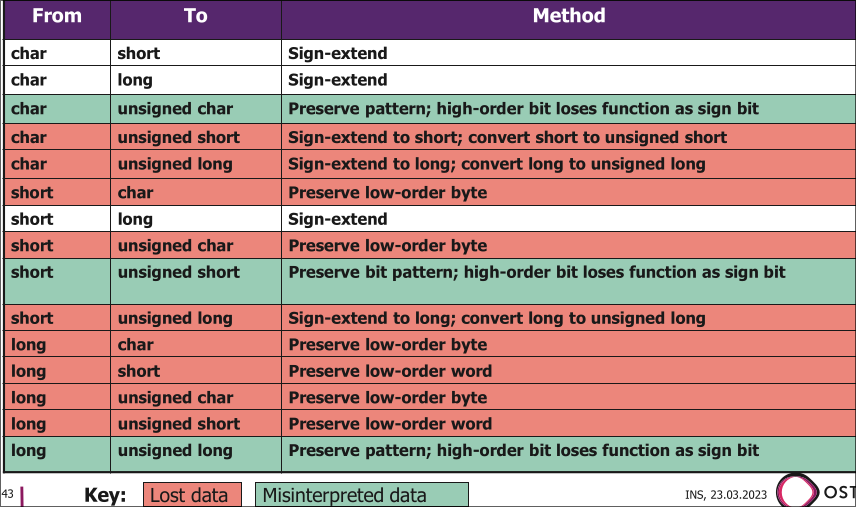
\includegraphics[scale=0.4]{2023_03_23_11_18_07.png}

\subsection{Examples for problems}

\subsubsection{Integer Overflow}
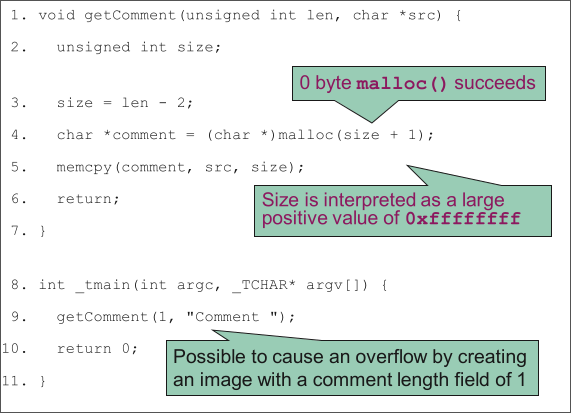
\includegraphics[scale=0.4]{2023_03_23_11_31_13.png}

\subsubsection{Sign Error}
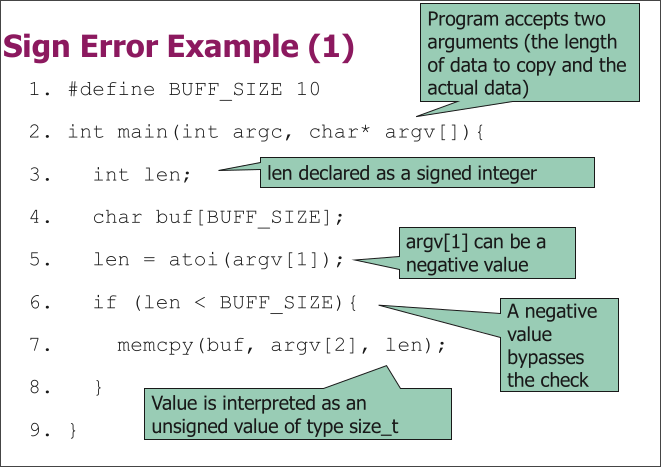
\includegraphics[scale=0.4]{2023_03_23_11_32_29.png}\newline
Problem: len is a signed integer, so it can be negative, but it is interpreted as size\_t when passed to memcpy!!

\subsubsection{Truncation}
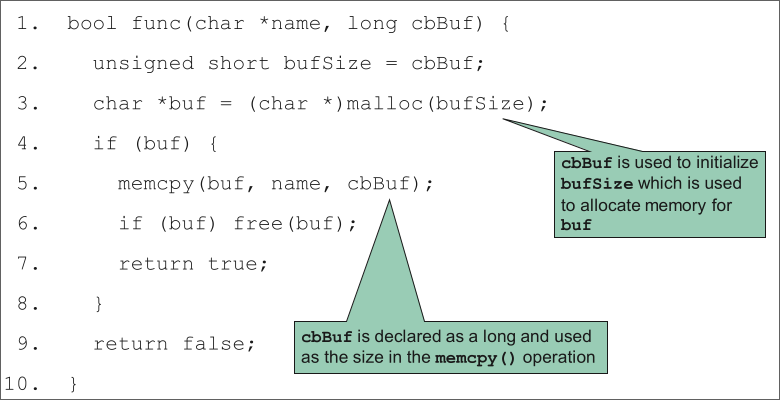
\includegraphics[scale=0.4]{2023_03_23_11_34_54.png}\newline
The value of bufSize might be trash since long is bigger than short, and it is unsigned, double fail!

\subsubsection{Negative Indices}
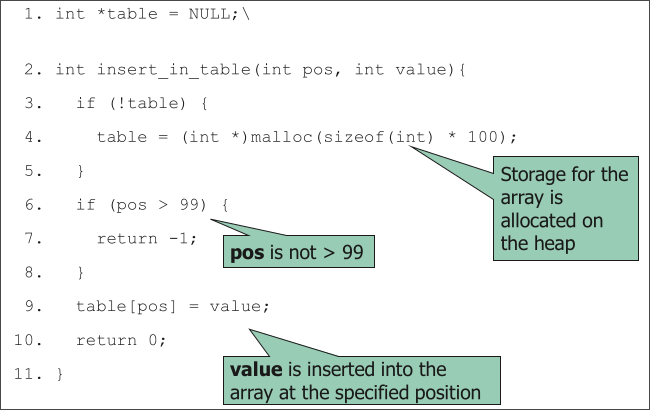
\includegraphics[scale=0.4]{2023_03_23_11_36_14.png}\newline
Negative indices will access previous values of the program, or cause a segfault when moving out of the program.

\subsection{Mitigations}
\begin{itemize}
\item \textcolor{purple}{Range checks for arrays etc}
\item \textcolor{purple}{Strong typechecks}
\item \textcolor{purple}{Abstract Data Types}
\item \textcolor{red}{USE FUCKING RUST}
\end{itemize} 

\section{Web Security}

\section{Reverse Engineering}

\subsection{Typical Problems}
Whenever we want to reverse engineer, we will walk into issues like \emph{obfuscation like mangling, or compressing of files}, all of these things will make it harder to de-compile and analyze the source.

\subsection{Example}
Here we would like to return true whether or not the key was right, we can do this by changing a line to xor instead of and:\newline
\includegraphics[scale=0.4]{2023_04_06_10_54_56.png}

\subsection{Mitigations}
\subsubsection{Anti-dissasebmly}
\begin{itemize}
\item \textcolor{black}{encrypted or packed code object}
\item \textcolor{black}{false dissasembly}
\item \textcolor{black}{self-modifying code}
\end{itemize} 
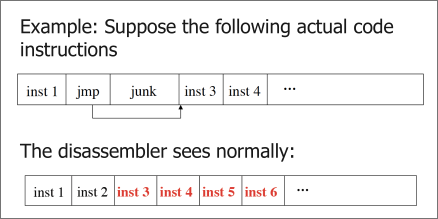
\includegraphics[scale=0.4]{2023_04_06_11_13_27.png}\newline
Essentially just insert garbage at a certain location.\newline
Can easily be dodged by noticing the jump.

\subsubsection{Anti-debugging techniques}
\begin{itemize}
\item \textcolor{black}{is\_debugger\_present() lmao}
\item \textcolor{black}{monitor for the use of debug registers and indserted breakpoints}
\item \textcolor{black}{use threads -> debuggers do not handle threads well}
\end{itemize} 
Debuggers often load instructions one by one, instead of all at once.\newline
Suppose we had a program where 4 instructions are loaded at once and later instruction 4 is overwritten with junk.\newline
This doesn't matter for the proper program, but it matters for the debugger, since it loads instruction in a serial manner.\newline
Regular mode:\newline
\includegraphics[scale=0.4]{2023_04_06_11_19_36.png}\newline
Debug mode: \newline
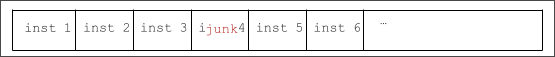
\includegraphics[scale=0.4]{2023_04_06_11_19_58.png}

\subsubsection{Tamper-resistance}
\begin{itemize}
\item \textcolor{black}{Make patching difficult}
\item \textcolor{black}{code is shown as hash -> needs to be processed first -> can have performance impacts}
\item \textcolor{black}{this approach is sometimes called "guards"}
\item \textcolor{black}{checks should not look similar, otherwise the protection is void}
\end{itemize} 

\subsubsection{Code obfuscation}
\begin{itemize}
\item \textcolor{black}{mangling}
\item \textcolor{black}{Code that is \emph{useless, or unused}, but hard to understand}
\item convert types like characters to ascii and back -> bruh
\end{itemize} 


\section{Secure Software Lifecycle}

\subsection{Three pillars for secure software}
\subsubsection{Risk Management}


\subsubsection{Touchpoints}


\subsubsection{Knowledge}



\section{Mobile Security}

\section{Security Testing}

\section{Bug Bounty}

\section{Software Security Assurance}

\section{Summary}

\end{document}
